\documentclass[11pt, a4paper]{article}
\usepackage[utf8]{inputenc}
\usepackage{listings}
\usepackage[margin=1.0in]{geometry}
\usepackage{color}
\usepackage{graphicx}
\usepackage{tabularx}
\usepackage{url}
\usepackage{float}
\usepackage{enumitem}
\usepackage{subcaption}

\lstnewenvironment{python}[1][]
{\lstset{
		language=python,
		numbers=left,
		numberstyle=\tiny,
		keywordstyle=\color{blue},       	% keyword style
		basicstyle=\footnotesize\ttfamily,	% font
		numbers=left,						% line numbers
		tabsize=2,							% tabsize in spaces
		#1}}
{}

\lstnewenvironment{bash}[1][]
{\lstset{
		language=bash,
		numbers=left,
		numberstyle=\tiny,
		numbers=none,
		basicstyle=\footnotesize\ttfamily,	% font
		tabsize=2,							% tabsize in spaces
		#1}}
{}

\lstnewenvironment{code}[1][]
{\lstset{numbers=left,
		numberstyle=\tiny,
		keywordstyle=\color{blue},       % keyword style
		basicstyle=\footnotesize\ttfamily,	% font
		numbers=left,						% line numbers
		tabsize=2,							% tabsize in spaces
		#1}}
{}

\title{DezSys06 - Verschlüsselung}
\author{Elias Frantar, Gary Ye (5AHITT)}
\date{\today{}, Wien}
\begin{document}

\lstset{
  backgroundcolor=\color{white},   % choose the background color; you must add \usepackage{color} or \usepackage{xcolor}
  basicstyle=\footnotesize,        % the size of the fonts that are used for the code
  breakatwhitespace=false,         % sets if automatic breaks should only happen at whitespace
  breaklines=true,                 % sets automatic line breaking
  captionpos=b,                    % sets the caption-position to bottom
% commentstyle=\color{mygreen},    % comment style
  deletekeywords={...},            % if you want to delete keywords from the given language
  escapeinside={\%*}{*)},          % if you want to add LaTeX within your code
  extendedchars=true,              % lets you use non-ASCII characters; for 8-bits encodings only, does not work with UTF-8
% frame=single,                    % adds a frame around the code
  keepspaces=true,                 % keeps spaces in text, useful for keeping indentation of code (possibly needs columns=flexible)
  keywordstyle=\color{blue},       % keyword style
% language=bash,                   % the language of the code
  morekeywords={*,...},            % if you want to add more keywords to the set
  numbers=none,                    % where to put the line-numbers; possible values are (none, left, right)
  numbersep=5pt,                   % how far the line-numbers are from the code
%  numberstyle=\tiny\color{gray}, % the style that is used for the line-numbers
  rulecolor=\color{black},         % if not set, the frame-color may be changed on line-breaks within not-black text (e.g. comments (green here))
  showspaces=false,                % show spaces everywhere adding particular underscores; it overrides 'showstringspaces'
  showstringspaces=false,          % underline spaces within strings only
  showtabs=false,                  % show tabs within strings adding particular underscores
%  stepnumber=1,                    % the step between two line-numbers. If it's 1, each line will be numbered
  stringstyle=\color{red},     % string literal style
  tabsize=2,                       % sets default tabsize to 2 spaces
  title=\lstname,                   % show the filename of files included with \lstinputlisting; also try caption instead of title
  belowskip=-3em,    
}

\setlength\parindent{0pt}

\maketitle
\newpage
\tableofcontents
\newpage

\section{Requirements}

\subsection{Kommunikation [12 Pkt]}

Programmieren Sie eine Kommunikationsschnittstelle zwischen zwei Programmen (Sockets; Übertragung von Strings). Implementieren Sie dabei eine unsichere (plainText) und eine sichere (secure-connection) Übertragung.
\\\\
Bei der secure-connection sollen Sie eine hybride Übertragung nachbilden. D.h. generieren Sie auf einer Seite einen privaten sowie einen öffentlichen Schlüssel, die zur Sessionkey Generierung verwendet werden. Übertragen Sie den öffentlichen Schlüssel auf die andere Seite, wo ein gemeinsamer Schlüssel für eine synchrone Verschlüsselung erzeugt wird. Der gemeinsame Schlüssel wird mit dem öffentlichen Schlüssel verschlüsselt und übertragen. Die andere Seite kann mit Hilfe des privaten Schlüssels die Nachricht entschlüsseln und erhält den gemeinsamen Schlüssel.

\subsection{Sniffer [4 Pkt]}

Schreiben Sie ein Sniffer-Programm (Bsp. mithilfe der jpcap-Library http://jpcap.sourceforge.net oder jNetPcap-Library http://jnetpcap.com/), welches die plainText-Übertragung abfangen und in einer Datei speichern kann. Versuchen Sie mit diesem Sniffer ebenfalls die secure-connection anzuzeigen.

\subsection{Info}

Gruppengröße: 2 Mitglieder \\
Punkte: 16

\begin{itemize}
	\item Erzeugen von Schlüsseln: 4 Punkte
	\item Verschlüsselte Übertragung: 4 Punkte
	\item Entschlüsseln der Nachricht: 4 Punkte
	\item Sniffer: 4 Punkte
\end{itemize}

\section{Effort Estimation and Work Distribution}

The following table compares the estimated with the actually needed
amount of time for completing each individual task.
\\\\
The estimation is in the second column while the columns that follow
are actual values.

\parskip 12pt
\begin{tabular} {| l | c | c | c | c |}
	\hline
	Task					&	Estimation		& 	Elias 	& 	Gary 	& 	Team	\\ \hline \hline
	Preparation				&					&			&  			&			\\ \hline
	Design					&					&			&			&			\\ \hline
	Implementation			&					&			&			& 	 		\\ \hline
	Testing					&					&			& 			& 	 		\\ \hline
	Documentation			&					&			&			& 			\\ \hline 
	Total					&					&			&			& 			\\
	\hline
\end{tabular}

\newpage

\section{Design}
\label{sec:design}

\subsection{Application Design}

\subsection{Encryption Parameters}

For symmetric encryption we decided to use the very standard \textit{AES} with
128 bit key- and block-size. We used the algorithm in \textit{Cipher Block
	Chaining (CBC)} mode with \textit{PKCS5} padding for messages which are too
short.
\\\\
For asymmetric encryption we used \textit{RSA} with \textit{PKCS1 Optimal
	Asymmetric Encrytpion Padding (OAEP)}. The keys are 2048 bits long and have a
public exponent of \textit{65537}.
\\\\
Both keys are generated by the cryptographically strong RNG implementation of
PyCrypto.

\subsection{Protocol Flaws \& Proposed Solutions}

The encryption protocol \textbf{was implemented as requested in the problem
	statement}. This protocol has some serious issues though:

\begin{description}
	
	\item[Man in the Middle Attacks] Since the public key is sent in plain
	without any certificates and signatures, it is incredibly easy for Eve to
	replace this key with her own and perform a full \textit{Man in the Middle}
	attack.
	
	\item[No Authentication] Both the key-exchange messages and the standard
	messages are sent without any type of authentication. This means that an
	attacker can arbitrarily modify them without being detected, which can
	lead to numerous very dangerous attacks.
	
	\item[Replay Attacks] Since messages are sent without any timestamps or
	message-counters Eve can easily resend messages at any time. This is
	negligible in comparison to the other flaws though.
	
\end{description}

Since the goal of this exercise was to get familiar with implementing crypto
and not to build a really secure application and due to time constraints, we
\textbf{decided not to fix this issues}.
\\\\
Here are some suggestions how we would have solved the above mentioned problems:

\begin{description}
	
	\item[Use TLS] The proposed protocol is just a minified and therefore very
	weak version of \textit{TLS}. So probably the easiest and \textbf{most
		secure} solution would be to use a tested common TLS implementation.
	
	\item[Use Digital Signatures] The only real way to prevent Man in the Middle
	attacks without \textit{real} certificates is to store public keys on the
	client side (copied before communication over a secure channel; ex. USB) and
	then send the keys in combination with a digital signature. The client can
	then verify this signature used one of the locally stored keys and therefore
	ensure that he is communication with the correct key owner.
	
	\item[Use MACs / or AES GCM-mode] The authentication issue could be resolved
	quite simply by applying a \textit{Message Authentication Code (MAC)} to
	each sent message. The same could be achieved by just using AES in
	\textit{Galois Counter Mode}.
	
	\item[Use Timestamps or Message Counters] The replay issue could be
	addressed by appending timestamps to messages or using counters to ensure
	that they are sent only once.
	
\end{description}

\subsection{IP and TCP protocol}
\label{subsec:iptcp}
Sniffing the packages is very simple, but interpreting them
appropriately is a completely different kettle of fish. 

The structure of the IP and the TCP headers were proposed in RFC 791
and RFC 793 respectively, but they can also be found below. 

For example, the IP header, as suggested in RFC 791 \cite{rfc791}, has
the following structure. 

%    IP Header (http://tools.ietf.org/html/rfc791):
\begin{lstlisting}
  0                   1                   2                   3
  0 1 2 3 4 5 6 7 8 9 0 1 2 3 4 5 6 7 8 9 0 1 2 3 4 5 6 7 8 9 0 1
  +-+-+-+-+-+-+-+-+-+-+-+-+-+-+-+-+-+-+-+-+-+-+-+-+-+-+-+-+-+-+-+-+
  |Version|  IHL  |Type of Service|          Total Length         |
  +-+-+-+-+-+-+-+-+-+-+-+-+-+-+-+-+-+-+-+-+-+-+-+-+-+-+-+-+-+-+-+-+
  |         Identification        |Flags|      Fragment Offset    |
  +-+-+-+-+-+-+-+-+-+-+-+-+-+-+-+-+-+-+-+-+-+-+-+-+-+-+-+-+-+-+-+-+
  |  Time to Live |    Protocol   |         Header Checksum       |
  +-+-+-+-+-+-+-+-+-+-+-+-+-+-+-+-+-+-+-+-+-+-+-+-+-+-+-+-+-+-+-+-+
  |                       Source Address                          |
  +-+-+-+-+-+-+-+-+-+-+-+-+-+-+-+-+-+-+-+-+-+-+-+-+-+-+-+-+-+-+-+-+
  |                    Destination Address                        |
  +-+-+-+-+-+-+-+-+-+-+-+-+-+-+-+-+-+-+-+-+-+-+-+-+-+-+-+-+-+-+-+-+
  |                    Options                    |    Padding    |
  +-+-+-+-+-+-+-+-+-+-+-+-+-+-+-+-+-+-+-+-+-+-+-+-+-+-+-+-+-+-+-+-+
\end{lstlisting}

And the TCP header, as suggested in RFC 793 \cite{rfc793}:

\begin{lstlisting}
  0                   1                   2                   3
  0 1 2 3 4 5 6 7 8 9 0 1 2 3 4 5 6 7 8 9 0 1 2 3 4 5 6 7 8 9 0 1
  +-+-+-+-+-+-+-+-+-+-+-+-+-+-+-+-+-+-+-+-+-+-+-+-+-+-+-+-+-+-+-+-+
  |          Source Port          |       Destination Port        |
  +-+-+-+-+-+-+-+-+-+-+-+-+-+-+-+-+-+-+-+-+-+-+-+-+-+-+-+-+-+-+-+-+
  |                        Sequence Number                        |
  +-+-+-+-+-+-+-+-+-+-+-+-+-+-+-+-+-+-+-+-+-+-+-+-+-+-+-+-+-+-+-+-+
  |                    Acknowledgment Number                      |
  +-+-+-+-+-+-+-+-+-+-+-+-+-+-+-+-+-+-+-+-+-+-+-+-+-+-+-+-+-+-+-+-+
  |  Data |           |U|A|P|R|S|F|                               |
  | Offset| Reserved  |R|C|S|S|Y|I|            Window             |
  |       |           |G|K|H|T|N|N|                               |
  +-+-+-+-+-+-+-+-+-+-+-+-+-+-+-+-+-+-+-+-+-+-+-+-+-+-+-+-+-+-+-+-+
  |           Checksum            |         Urgent Pointer        |
  +-+-+-+-+-+-+-+-+-+-+-+-+-+-+-+-+-+-+-+-+-+-+-+-+-+-+-+-+-+-+-+-+
  |                    Options                    |    Padding    |
  +-+-+-+-+-+-+-+-+-+-+-+-+-+-+-+-+-+-+-+-+-+-+-+-+-+-+-+-+-+-+-+-+
  |                             data                              |
  +-+-+-+-+-+-+-+-+-+-+-+-+-+-+-+-+-+-+-+-+-+-+-+-+-+-+-+-+-+-+-+-+
\end{lstlisting}

\lstinline|data| is, as the name suggests, the content of the package,
and will contain the plain text, or cipher text in our exercise. 

\section{Implementation}

\subsection{Crypto}

Our library of choice for Python was PyCrypto \cite{pycrypto}. Installation works quick and easy via \lstinline|pip| or \textit{PyCharm}.
\\\\
This section briefly describes how to perform crypto primitives such as key-generation, en- and decryption in PyCrypto.
Our full implementations are included in \lstinline|symmetric.py| and \lstinline|asymmetric.py| (\lstinline|spychat/crypto/|).

\subsubsection{Key Generation}

For generating encryption keys cryptographically strong key-generation algorithms are crucial. PyCrypto provides one-liner functions to generate secure keys for symmetric and asymmetric encryption algorithms.

\vspace{5pt}
\begin{python}
# asymmetric key-generation
RSA.generate(RSA_KEY_LEN_BITS, e=RSA_E)

# symmetric key-generation
Random.new().read(AES_KEY_LEN)
\end{python}
\vspace{10pt}

For creating RSA keys a specific function can be used to generate keys of desired length. Symmetric encryption keys can be generated with PyCrypto's general secure random class \lstinline|Random|.

\subsubsection{En- \& Decryption}

PyCrypto also provides a very easy to use interface for RSA encryption.

\vspace{5pt}
\begin{python}
	RSA_MODE = PKCS1_OAEP
	
	# asymmetric encryption
	rsa = RSA_MODE.new(public_key)  # `keypair.publickey()`
	rsa.encrypt(data)
	
	# asymmetric decryption
	rsa = RSA_MODE.new(private_key)
	return rsa.decrypt(data)
\end{python}
\vspace{10pt}

It classes for the different padding-mode, which instances can be intuitively used for performing crypto operations after passing the appropriate keys. We chose \textit{PKCS1\_OAEP} mode since this pretty much the best mode to use for RSA.
\\\\
Symmetric encryption is a bit hard in PyCrypto, since it \textit{does not implement automatic padding}. We therefore had to write our own \textit{PKCS5} padding function.

\vspace{5pt}
\begin{python}
# PKCS5 padding implementation
def pad(data):
	pad_nr = AES_BLOCK_SIZE - (len(data) % AES_BLOCK_SIZE)
	return data + (chr(pad_nr) * pad_nr)
def unpad(data):
	return data[:len(data) - data[-1]]
\end{python}
\vspace{10pt}

This type of padding simply repeats the numbers of missing bytes to fill up to the block-length.
\\\\
With this function symmetric encryption and decryption isn't much harder either, except that \textit{IVs must randomly generated and prepended to the ciphertext for security reasons.}

\vspace{5pt}
\begin{python}
# symmetric encryption
iv = Random.new().read(AES_BLOCK_SIZE)

aes = AES.new(key, AES_MODE, iv)
return iv + aes.encrypt(pad(data))

# symmetric decryption
iv = data[:AES_BLOCK_SIZE]
data = data[AES_BLOCK_SIZE:]

aes = AES.new(key, AES_MODE, iv)
return unpad(aes.decrypt(data))
\end{python}
\vspace{10pt}

IVs can be created similar to symmetric keys with \lstinline|Random|. They must then be prepended to the ciphertext after encryption and removed and passed to algorithm before decryption. It is also necessary to pad data to the appropriate block-size before encryption (and remove it after decryption of course).

\subsection{Sniffer}

We implemented the sniffer by considering every sent and received
package, and parsing them appropriately according to the scheme as
already described in \ref{subsec:iptcp}. The idea of this low level
implementation comes from an online article \cite{sniffer_py} that
suggests decoding the raw packages without using any external
libraries like \textit{pcap}.

Merely using the following Python code results to a powerful sniffer
that can be extended by parsing the raw data accordingly. 

\begin{python}
import socket
 
# create an INET, raw socket
s = socket.socket(socket.AF_INET, socket.SOCK_RAW, socket.IPPROTO_TCP)

# receive a packet
while True:
  print s.recvfrom(65565)
\end{python}

The description of our sniffer follows, and we begin by alluding that
the following program instructions are done in an endless while loop.

We first assign the raw packet \lstinline|bytes| by taking the first
element of the tuple that the \lstinline|recvfrom()| method returns. 

\begin{python}
# We will receive the packet 
packet = s.recvfrom(65565)[0]
\end{python}

Afterwards, we \textit{unpack} the raw packet by:

\begin{enumerate}
  \item only considering the first 20 bytes of the packet since these
    are the header bytes of the IP protocol. 
  \item unpacking the bytes with the \lstinline|struct.unpack|
    method according to the ``!BBHHHBBH4s4s'' scheme. In this scheme
    the meanings of the characters are:
    
    \begin{itemize}
      \item ! meaning this is a network package (=big endian)
      \item B for unsigned char (1 byte)
      \item H for unsigned short (2 byte)
      \item 4s for char[4] which will just be interpreted as
        \lstinline|str| in Python
    \end{itemize}
    The unpack method returns a list with the data in the
    corresponding indices e.g. list[2] stands for the first unsigned
    short according to the scheme. 
\end{enumerate}

\begin{python}
iph = unpack('!BBHHHBBH4s4s' , packet[0:20])
\end{python}

Next, we find out the IHL (IP Header Length) according to
\ref{subsec:iptcp}, by taking the first byte, and only considering the
last four bits of it. Denote $x$ as the 4 bit integer that is written
in the IHL. By the definition of RFC791\cite{rfc791}, we know that the
whole IP header length consists of $x \cdot 32$ bits, thus knowing
where to start looking for the header of the corresponding protocol
e.g. TCP header - see below for more information.

The version of the package is irreleveant because we always assume for
the range of this exercise that IPV4 packages are being exchanged.

\begin{python}
version_ihl = iph[0]
version = version_ihl >> 4
ihl = version_ihl & 0xF

iph_length = ihl * 4
\end{python}

The protocol should have the value 6, which is also the value for TCP
protocol. In this exercise, we only filter out TCP packages, but we
also assume that TCP packages are solely exchanged. 

\begin{python}
protocol = iph[6]
\end{python}

Next, we convert the source and destination address by using the
\lstinline|socket.inet_ntoa| method. The addresses can be used for
filtering purposes. 

\begin{python}
src_addr = socket.inet_ntoa(iph[8]);
dst_addr = socket.inet_ntoa(iph[9]);
\end{python}

Now that the most essential information are read we can continue by
reading the TCP header. The scheme for reading the data is similiar to
above that's why, only the code will be shown below. 

\begin{python}
tcp_header = packet[iph_length:iph_length+20]
tcph = unpack('!HHLLBBHHH' , tcp_header)

src_port = tcph[0]
dst_port = tcph[1]
doff_reserved = tcph[4]
tcph_length = doff_reserved >> 4

h_offset = iph_length + tcph_length * 4
data = packet[h_offset:]
\end{python}


RFC793 \cite{rfc793} states:

\begin{quote}
\textit{Data Offset} is the number of 32 bit words in the TCP Header.
This indicates where the data begins.  The TCP header (even one
including options) is an integral number of 32 bits long.
\end{quote}

The actual content of the packet is stored in \lstinline|data|, and it
should be clear why. 

\section{Testing}

For validating the correctness of the programs we performed some
manual tests that will be described below. The tests were executed on
a Ubuntu 14.04 machine. 

The setup of the test was based on a real life scenario in which two
partners, say Alice and Bob, want to communicate privately through a
channel. The communication was done through a secure and an unsecure
channel, where the former one uses a certain encryption protocol, as
described in \ref{sec:design}, and the latter uses no particular
techniques for exchanging messages.

\begin{figure}[H]
  \centering
  \begin{subfigure}[b]{0.49\textwidth}
    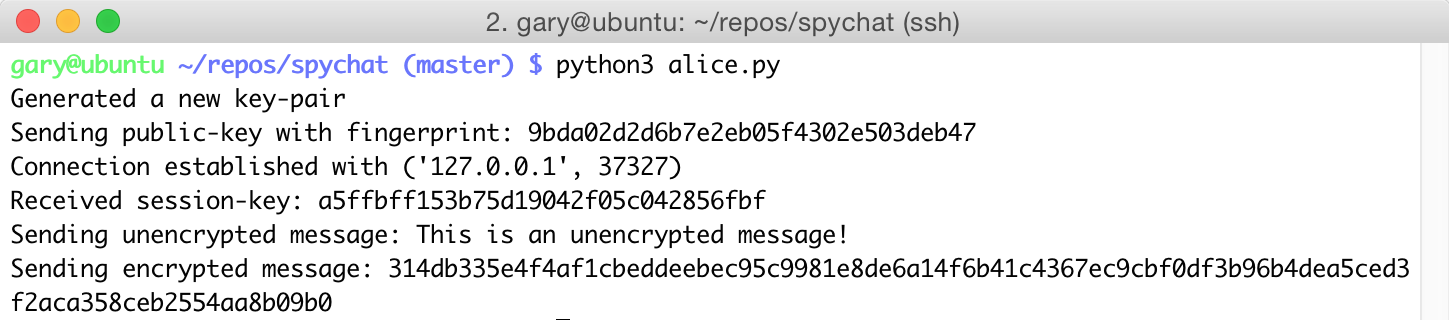
\includegraphics[width=\linewidth]{img/test_alice}
    \caption{Alice}
    \label{fig:test_alice}
  \end{subfigure}
  \begin{subfigure}[b]{0.49\textwidth}
    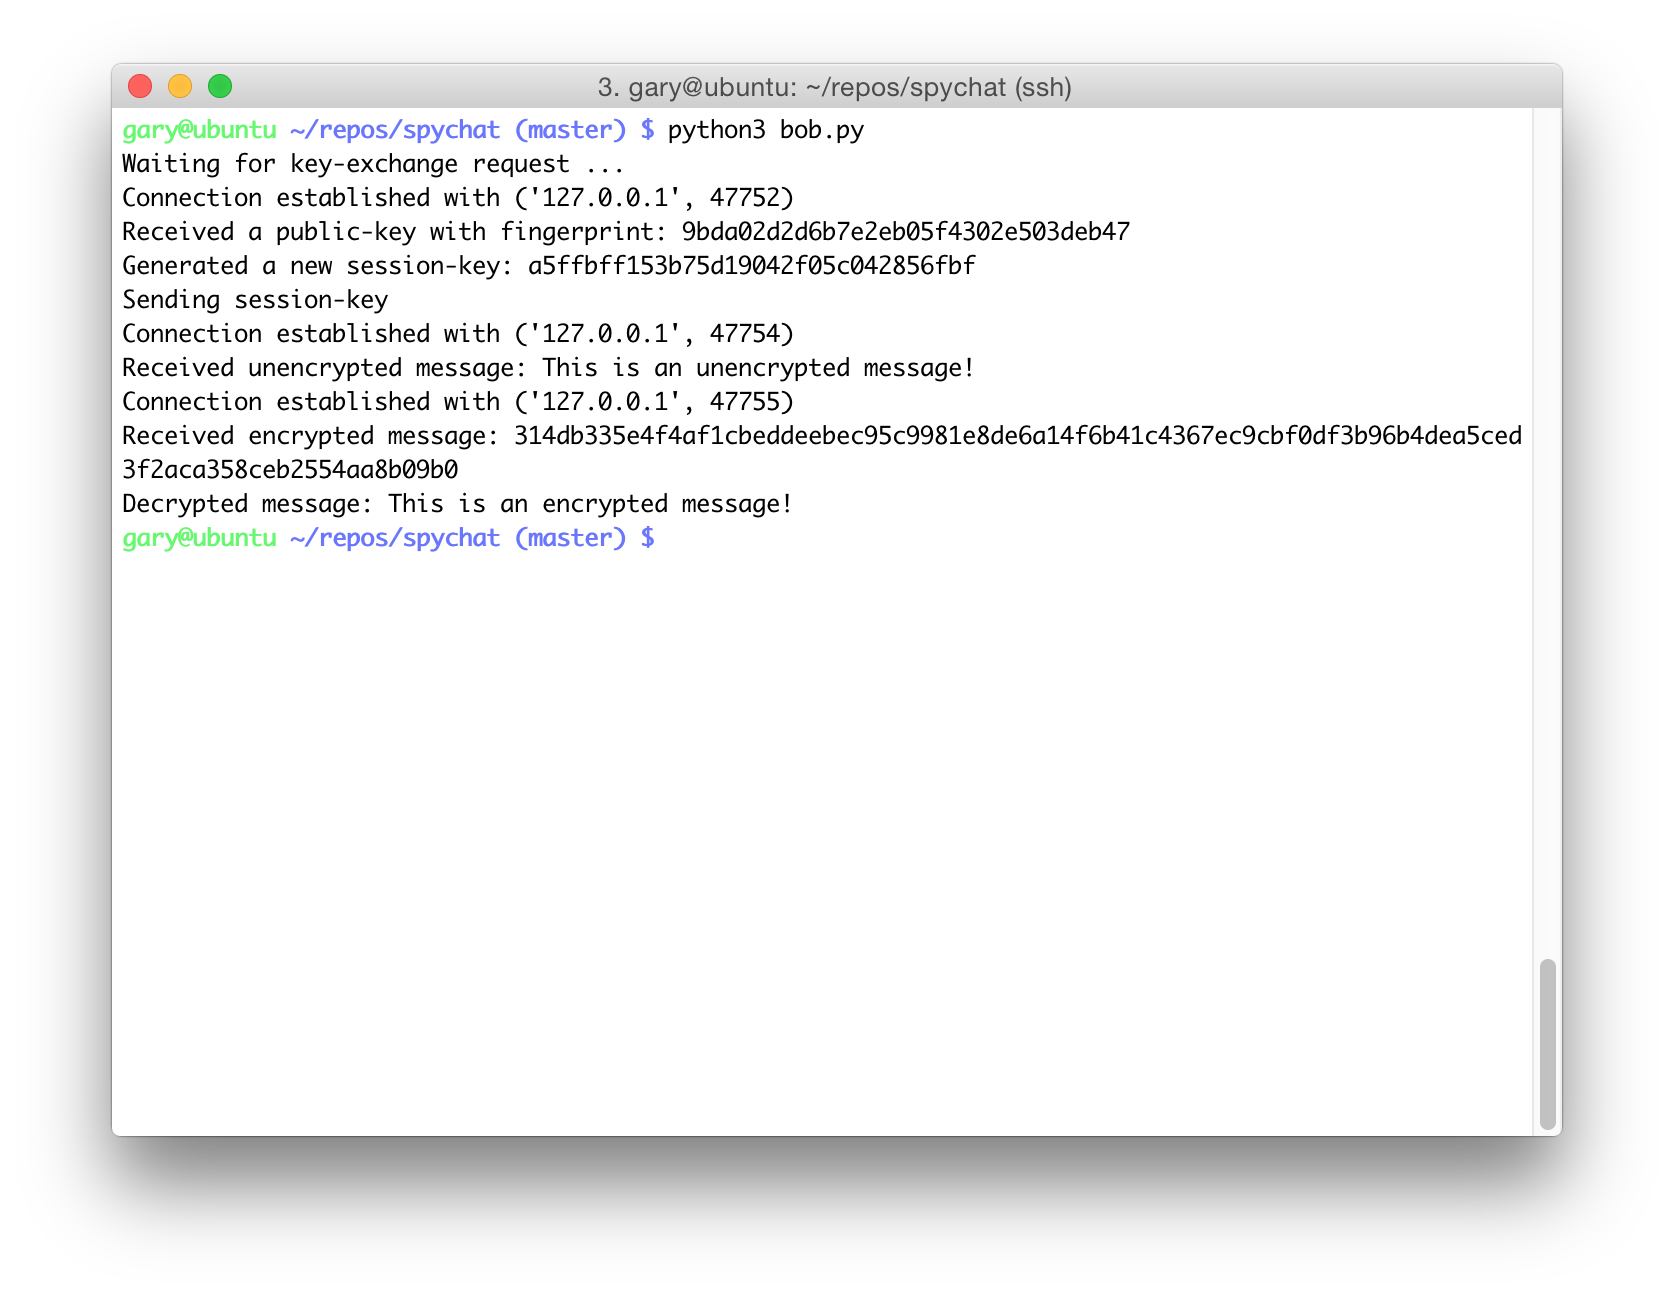
\includegraphics[width=\textwidth]{img/test_bob}
    \caption{Bob}
    \label{fig:test_bob}
  \end{subfigure}
\end{figure}

While Alice and Bob are chatting, Eve was eavesdropping them by using
the sniffer which was also implemented throughout this exercise. We
can see in Figure \ref{fig:test_eve} the messages, or rather the TCP
packets, that were exchanged during the communication process. 

For the sake of clarity, the most essential part of the TCP headers
are printed e.g. \lstinline|src_addr|, \lstinline|dst_addr|,
\lstinline|src_port|, \lstinline|dst_port|. The arguments that were
passed to the sniffer are the portnumbers that are interesting for the
user of the script. Only the given ones will be printed out to the
console, and the others will be omitted. 

It can be seen that the public key of Alice has been successfully
eavesdropped, and it was printed out in plaintext. Afterwards, we can
see the encrypted session key beginning that cannot be successfully
read, as we can see in the lower center of Figure \ref{fig:test_eve}. 

Aftewards two messages were exchange. The first one is simply
plaintext, and the second one was the message encrypted with the AES
session key. 

\begin{figure}[H]
  \centering
  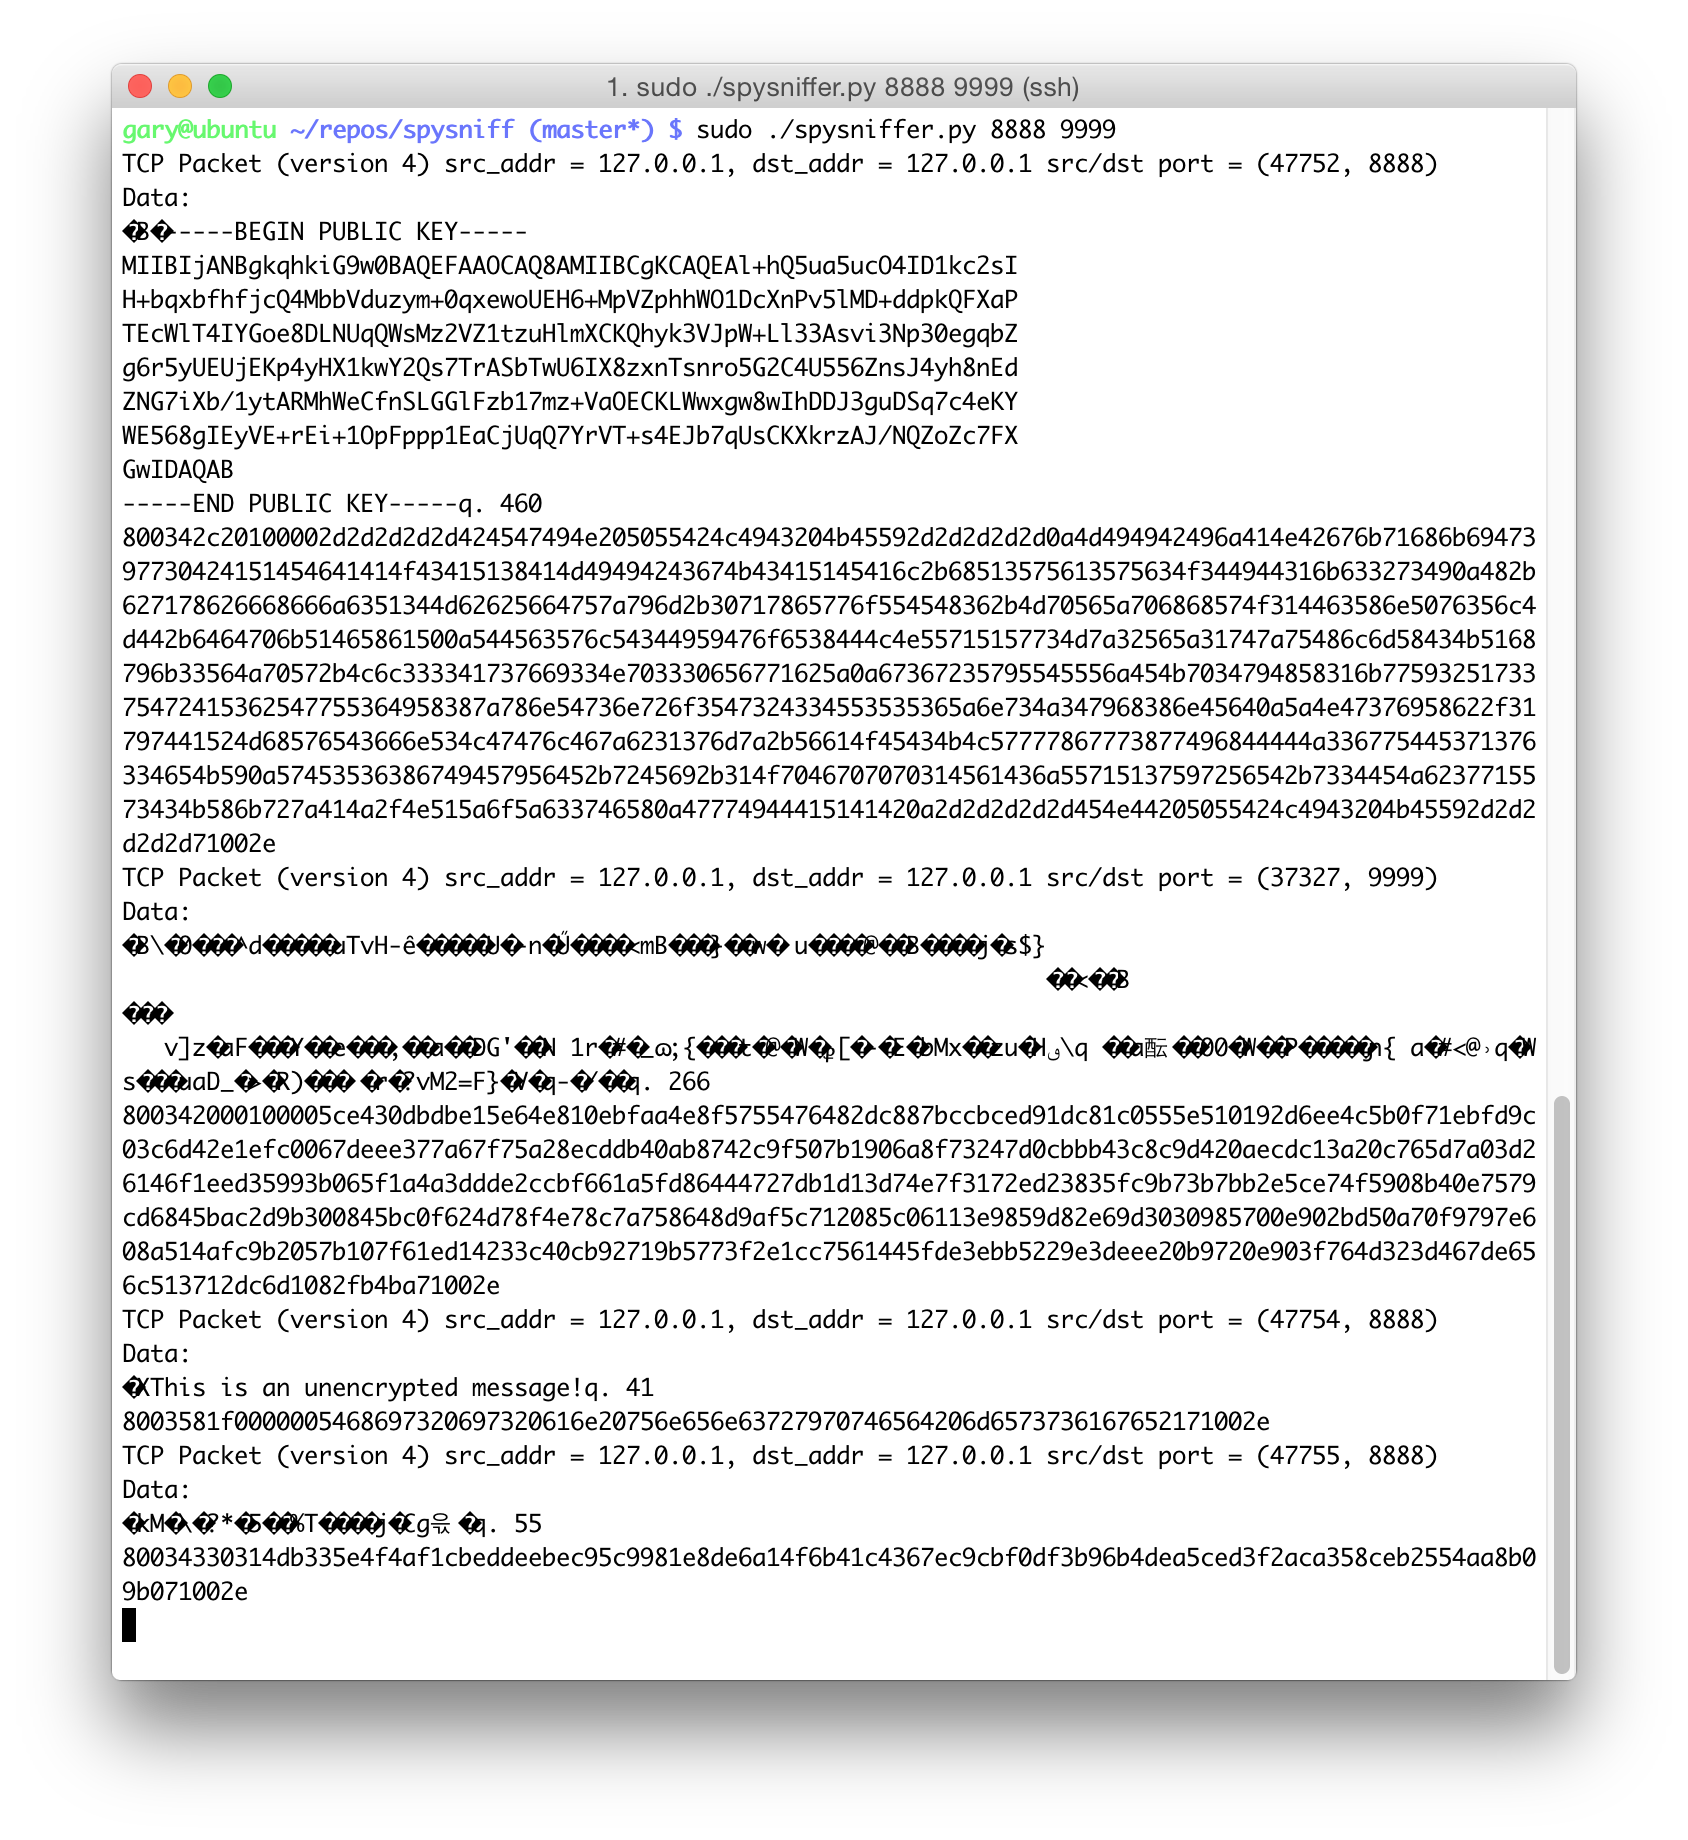
\includegraphics[width=0.8\linewidth]{img/test_eve}
  \caption{Eve}
  \label{fig:test_eve}
\end{figure}

\section{Problems \& Solutions}

\subsection{PyCrypto AES Counter Mode}

We originally wanted to used CTR mode for AES to avoid having to implement
padding. For some reason the CTR PyCrypto interface is really obscure and we
did not manage to get it working.
\\\\
So we simply switched to CBC and quickly implemented PKCS5 padding.

\subsection{Sending Public Keys}

Sending public keys (\lstinline{keypair.publickey()} generated by PyCrypto
proved to be an pretty odd problem because when trying to use the
\textit{properly} received keys for encryption, it caused an Exception that
some kind of random function is not defined.
\\\\
It turned out that public key objects are not meant to be sent around and
therefore have to be exported to a transmittable format beforehand. The above
code works fine:

\begin{lstlisting}
# `PEM` is just some standardized RSA-key format
pub_key = RSA.exportKey(keypair.publickey(), 'PEM')

# send `pub_key`

pub_key = RSA.importKey(received_key)
\end{lstlisting}

\nocite{*}
\bibliographystyle{plain}
\bibliography{bibliography}

\end{document}
